\begin{figure*}[t!]
\centering
\setcounter{subfigure}{0}
\subfigure[]
{
	\label{fig:berkeley_random_hum}
%	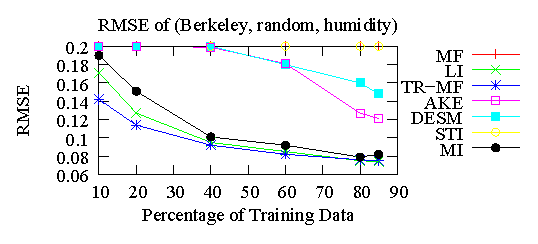
\includegraphics[height=2.5cm, trim=15 0 0 0, clip]{table2_1_BRH.eps}
	\includegraphics[height=2.8cm]{new/humidv3_5000_85_10_5_1.eps}
}
\hspace{0in}
%\end{figure}
%\begin{figure}[H]
%\centering
\subfigure[]
{
	\label{fig:berkeley_random_light}
	\includegraphics[height=2.8cm]{new/lightv3_5000_85_10_5_2.eps}
}
\hspace{0in}
%\caption{}
%\end{figure}
%\begin{figure}[H]
%\centering
\subfigure[]
{
	\label{fig:berkeley_random_tem}
	\includegraphics[height=2.8cm]{new/tempv3_5000_85_10_5_3.eps}
}
\hspace{0in}
%\caption{}
%\end{figure}
%\begin{figure}[H]
%\centering
\subfigure[]
{
	\label{fig:traffic_random_hum}
	\includegraphics[height=2.8cm]{new/traffic_v1_humid_43968_85_10_5_1.eps}
}
\hspace{0in}
%\caption{}
%\end{figure}
%\begin{figure}[H]
%\centering
\subfigure[]
{
	\label{fig:traffic_random_tem}
	\includegraphics[height=2.8cm]{new/traffic_v1_temp_43968_85_10_5_2.eps}
}
%\caption{Random Split}
\hspace{0in}
%\caption{}
%\end{figure*}
%\begin{table*}
%%
%\begin{tabular}{cc}
%\subfigure[A]{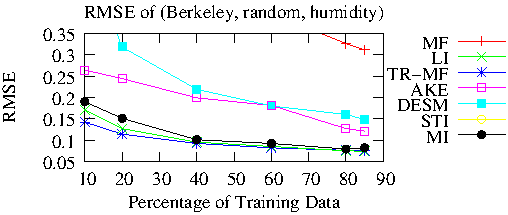
\includegraphics[height=2.5cm, trim=15 0 0 0, clip]{table2_BRH}} 
%   & \subfigure[B]{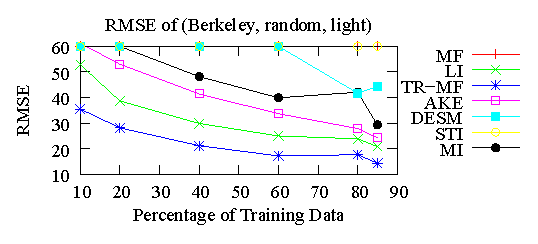
\includegraphics[height=2.5cm, trim=15 0 0 0, clip]{table3_BRL}}\\
%\end{tabularx}
%\end{table*}
%\end{figure}
%\begin{figure}[H]
%\centering
%\mbox{
%\input{table11.pspdftex}}
%\caption{RMSE of (traffic, temporal, temperature}
%\end{figure}
%\begin{figure*}[htbp]
%\centering
\subfigure[]
{
	\label{fig:berkeley_temporal_hum}
	\includegraphics[height=2.8cm]{new/humidv3_5000_85_10_5t_1.eps}
}
\hspace{0in}
%\end{figure}
%\begin{figure}[H]
%\centering
\subfigure[]
{
	\label{fig:berkeley_temporal_light}
	\includegraphics[height=2.8cm]{new/lightv3_5000_85_10_5t_2.eps}
}
\hspace{0in}
%\caption{}
%\end{figure}
%\begin{figure}[H]
%\centering
\subfigure[]
{
	\label{fig:berkeley_temporal_tem}
	\includegraphics[height=2.8cm]{new/tempv3_5000_85_10_5t_3.eps}
}
\hspace{0in}
\subfigure[]
{
	\label{fig:traffic_temporal_hum}
	\includegraphics[height=2.8cm]{new/traffic_v1_humid_43968_85_10_5t_1.eps}
}
\hspace{0in}
\subfigure[]
{
	\label{fig:traffic_temporal_tem}
	\includegraphics[height=2.8cm]{new/traffic_v1_temp_43968_85_10_5t_2.eps}
}
\hspace{0in}
\vspace{-0.1in}

\caption{Root mean square errors (RMSE) of models, varying the percentage of training data. 
%(a) to (d) are for random missing data; (e) to (h) are for consecutive missing data. 
We put a large asteroid symbol when TR-MF is significantly better than all the other models.
The units of measurement are Celsius for temperature, \% for humidity and lux for light.
}
\hspace{0in}
%\caption{}
\end{figure*}
